\section{Application to Langevin dynamics}
\label{sec:numerical_lang}
%
To illustrate the theoretical results obtained in \cref{sec:transient}, we apply the transient subtraction technique to compute the mobility and shear viscosity for a Lennard--Jones fluid, and to a low-dimensional example, with the Langevin dynamics \eqref{eq:lang_dynamics} serving as the underlying dynamics for all cases. We present our numerical results in three parts:
%
\begin{itemize}
	\item In \cref{subsec:num_lang}, we formulate the transient subtraction technique for Langevin dynamics by making precise $\varphi_1$ and $\varphi_2$ for the conjugate responses $S$ of interest.
%	 \item In \cref{subsec:num_1D}, we illustrate the results from \cref{prop:gen_subtraction} with the one-dimensional Langevin dynamics. The aim is to numerically present \eqref{eq:prop_eta_bias_bound}, the scaling of the $\eta$ bias for first and second-order maps $\Phi_\eta^\alpha$. The low dimensionality of the system in consideration allows us to compute \eqref{eq:prop_eta_bias_bound} directly at the level of operators.
	 \item In \cref{subsec:num_1D}, we numerically illustrate the finite $\eta$ bias results from \cref{cor:gk_equiv}, which apply~\eqref{eq:prop_eta_bias_bound} to the subtraction estimator \eqref{eq:ts_estimator}. In particular, we demonstrate the bias scaling for first and second-order maps $\Phi_\eta^\alpha$. This is done with the one-dimensional Langevin dynamics, which allows to directly compute \eqref{eq:prop_eta_bias_bound}, at the level of operators, by discretizing the associated PDE. This enables a clear and effective presentation of the result, which would have otherwise been challenging to achieve with usual stochastic approaches. %\red{reread}
	 \item Finally, we compute in \cref{subsec:num_LJ} the mobility and shear viscosity for a Lennard--Jones fluid. This aim is to demonstrate the usefulness and viability of the method in more practical, high-dimensional molecular dynamics settings, particularly by highlighting its variance reduction capabilities.
%
%	 \item Finally, we compute in \cref{subsec:num_LJ} the mobility and shear viscosity for a Lennard--Jones fluid to show applications of the subtraction technique to more practical, high-dimensional molecular dynamics systems, demonstrating the usefulness and practicality of the method, and especially to highlight its variance-reduction capabilities.
\end{itemize}

% ===================================================================================
%\subsection{Mobility and shear viscosity for Langevin dynamics}
%\label{subsec:num_mob_sv}
%
% ===================================================================================
\subsection{Transient methods for Langevin dynamics}
\label{subsec:num_lang}
%
%\subsubsection{Physical context}
%\label{subsubsec:physical_context}
%
Although our transient method only considers equilibrium dynamics, it encodes the relevant nonequilibrium information through the conjugate  response function $S$, which is the key quantity allowing to obtain the transport coefficient. This is expressed through the first-order perturbation PDE \eqref{eq:varphi1_PDE}, whose solution depends on $S$. To define it, let $F(q) \in \R^{d}$ represent an external forcing, chosen appropriately based on the transport coefficient in consideration. Particular choices for $F(q)$ are made precise for each scenario we consider in~\cref{subsec:num_LJ}. For all such scenarios, the associated conjugate response function $S$ is given by
%
\begin{equation}
    S(q,p) = \beta F(q)^\t M^{-1} p.
    \label{eq:conj_res}
\end{equation}
%
We remark that the formal definition of $S$ is based on the associated nonequilibrium dynamics, and relies on linear response theory to be rigorously derived. In the interest of clarity, we do not provide such a rigorous discussion, and instead refer the reader to \cite[Section 5.2.3]{lelievre2016} for a comprehensive discussion.

Having identified the appropriate conjugate response function~$S$, one can now construct the map~$\Phi_\eta^\alpha$, for~$\alpha=1,2$, by solving the associated PDEs~\eqref{eq:varphi1_PDE} and~\eqref{eq:varphi2_PDE}. 
%It is often the case that the nongradient force $F(q,p)$ used to compute transport coefficients in NEMD is divergence-free. In particular, this holds for the examples we consider here, made precise in \eqref{subsec:num_mob_sv}, so we have that $S = \beta p^\t M^{-1} F(q)$.
%
%\begin{equation}
%	S = \beta F^\t M^{-1}p.
%\end{equation}
%

\paragraph{First-order map $\varphi_1$} For convenience, let us first recall the expression for \eqref{eq:varphi1_PDE}: %\red{$d$ and $x$ vs $q,p$ for langevin below}
%
\begin{equation}
	\nabla^*\varphi_1 = \sum_{i=1}^d \partial_{x_i}^* \varphi_{1,x_i} = S. %-\div(\varphi_1) + \beta\nabla U\varphi_1 = S
\end{equation}
%
For Langevin dynamics, it is natural to consider the position and momentum components of $\varphi_1$ by writing $\varphi_1(q,p) = (\varphi_{1,q}(q,p), \varphi_{1,p}(q,p))$, so that we can write $\nabla^*\varphi_1 = \nabla^*_q\varphi_{1,q} + \nabla^*_p\varphi_{1,p}$. More precisely, the action of the adjoint operators are given by
%
\begin{equation}
	\partial^*_{q_i} = - \partial_{q_i} + \beta\partial_{q_i} V , \qquad \partial^*_{p_i} = - \partial_{p_i} + \beta (M^{-1}p)_i,
	\label{eq:nabla_star_expressions}
\end{equation}
%
which can be obtained via integration by parts as in \eqref{eq:Astar_adjoint}. In view of \eqref{eq:nabla_star_expressions} and \eqref{eq:conj_res}, we can write~\eqref{eq:varphi1_PDE} more explicitly for Langevin dynamics as
%
\begin{equation}
	-\Div_q(\varphi_{1,q}) - \Div_p(\varphi_{1,p}) + \beta \nabla V^\t \varphi_{1,q} + \beta p^\t M^{-1} \varphi_{1,p} = \beta F(q)^\t M^{-1} p.
\end{equation}
%
Therefore, a natural solution for \eqref{eq:varphi1_PDE} in any dimension is
%
\begin{equation}
	\varphi_1(q,p) = \begin{pmatrix}
 	\varphi_{1,q}(q,p) \\ \varphi_{1,p}(q,p)
 	\end{pmatrix} =
	\begin{pmatrix}
 	0 \\ F(q)
 	\end{pmatrix},
 	\label{eq:varphi1_sol}
\end{equation}
%
and the transformation $\Phi^1_\eta$ is then given by
%
\begin{equation}
	\Phi_\eta^1(q,p) = 
	\begin{pmatrix}
 	  q \\ p + \eta F(q)
 	\end{pmatrix}.
\end{equation}
%
Thus, constructing the initial conditions for a first-order transient trajectory simply amounts to shifting the initial momentum $p_0^0$ of some associated stationary equilibrium process by $\eta F(q_0^0)$.

\paragraph{Second-order map $\varphi_2$} Constructing the second-order map amounts to finding~$\varphi_2$ by solving~\eqref{eq:varphi2_PDE}, which we recall for convenience:
%
\begin{equation}
	\nabla^*\varphi_2 = -\frac{1}{2}\sum_{i,j=1}^d \partial_{x_i}^*\partial_{x_j}^* (\varphi_{2,x_i}\varphi_{2,x_j}) = -\frac{1}{2}(\nabla^*)^2 \colon \varphi_1\otimes \varphi_1.
\end{equation}
%
Substituting the solution \eqref{eq:varphi1_sol} for $\varphi_1$ in \eqref{eq:varphi2_PDE} leads to
%
\begin{align}
    \nabla^*\varphi_2 &= -\frac{1}{2}(\nabla^*)^2\colon 
    \begin{pmatrix}
        0 \\ F    
    \end{pmatrix} \otimes 
    \begin{pmatrix}
        0 \\ F    
    \end{pmatrix} \equiv -\frac{1}{2}(\nabla_p^*)^2 \colon F\otimes F.
\end{align}
%
Thus, as in the first-order case, one can choose $\varphi_{2,q} = 0$ so that $\varphi_2 = (0, \varphi_{2,p}(q,p))$. Next, recalling that~$\partial^*_{p_i} = -\partial_{p_i} - \beta (M^{-1}p)_i$,
%
\begin{align}
    -\frac{1}{2}(\nabla_p^*)^2 \colon F\otimes F &= -\frac{1}{2}\sum_{i,j=1}^d \partial_{p_i}^*\partial_{p_j}^* \paren*{F_i F_j} \\
    &= -\frac{\beta}{2}\sum_{i,j=1}^d \bkt*{-\partial_{p_i} + \beta (M^{-1}p)_i}(M^{-1}p)_j F_i F_j \\
    &= -\frac{\beta^2}{2}\sum_{i,j=1}^d (M^{-1}p)_i(M^{-1}p)_j F_i F_j + \frac{\beta}{2} \sum_{i,j=1}^d \partial_{p_i}(M^{-1}p)_j F_iF_j \\
    &= -\frac{\beta^2}{2}\sum_{i,j=1}^d (M^{-1}p)_i(M^{-1}p)_j F_i F_j +\frac{\beta}{2}\sum_{i,j=1}^d M^{-1}_{j,i} F_i F_j \\
    &= -\frac{1}{2}\paren*{\beta p^\t M^{-1}F}^2 + \frac{1}{2}\beta F^\t M^{-1}F.
    %\equiv \nabla^*\varphi_2.
\end{align}
%
Thus, a possible solution for the second-order term $\varphi_2$ is
%
\begin{equation}
    \varphi_2(q,p) = 
    \begin{pmatrix}
        0 \\ -\dfrac{\beta F(q)^\t M^{-1} p}{2}F(q)
    \end{pmatrix} = 
    \begin{pmatrix}
        0 \\ -\dfrac{1}{2}S(q,p)F(q)
    \end{pmatrix}.
\end{equation}
%
This leads to the second-order transformation $\Phi_\eta^\alpha$
%
\begin{equation}
	\Phi_\eta^2(q,p) = 
	\begin{pmatrix}
 	  q \\ p + \eta F(q) - \dfrac{\eta^2}{2}F(q)S(q,p)
 	\end{pmatrix}.
\end{equation}
%
\begin{comment}
%
\begin{align}
	\nabla^*\varphi_2 &= \partial_p^*(\varphi_{2,p}) \\
	&= -\frac{1}{2\beta^2}(\partial_p^*)^2(F(q)^2) \\
	&= -\frac{1}{2\beta}\partial_p^*(pF(q)^2) \\
	&= -\frac{1}{2}\paren*{p^2 - \frac{1}{\beta}}F(q)^2.
\end{align}
%
Thus, we obtain
%
\begin{equation}
	\varphi_2 = \begin{pmatrix}
		0 \\ -\frac{p}{2\beta}F(q)^2
	\end{pmatrix}
\end{equation}
\end{comment}

%\begin{table}[tbhp]
%\begin{center}
%	\begin{tabular}{lccc} 
%	\hline\hline
%	\bf{Parameter} & {\bf 1D Lang.} & {\bf Shear visc.} & {\bf Mobility} \\
%	\hline
%%	Perturbation $\eta$ & $10^{-2}$ & $10^{-2}$ & $10^{-2}$ \\
%	Replicas $K$ & $10^6$ & $10^5$ & $10^5$ \\
%	Timestep $dt$ & $10^{-2}$ & $10^{-2}$ & $10^{-2}$ \\
%	Inverse temp. $\beta$ & 1 & 1.25 & 0.8 \\
%	Damping $\gamma$ & 1 & 1 & 1 \\
%	No. of particles $N$ & 1 & 1000 & 1000 \\
%	Density $\varrho$ ($N$/vol.) & - & 0.7 & 0.6 \\
%	LJ cutoff $r_\mathrm{c}$ & - & 2.5 & 2.5 \\
%	\hline
%	\end{tabular}
%\end{center}
%\caption{Simulation parameters}
%\label{table:sim_params}
%\end{table}
% ===================================================================================
\subsection{One-dimensional Langevin dynamics}
\label{subsec:num_1D}
%
%
%\begin{align}
%%    \begin{pmatrix}
%%        q_0^\eta \\ p_0^\eta
%%    \end{pmatrix}
%	 = \Phi_\eta(q_0^0,p_0^0) = 
%	\begin{pmatrix}
% 	  q_0^0 \\ p_0^0 + \eta
% 	\end{pmatrix}
%\end{align}
%\begin{align}
%    (q_0^\eta, p_0^\eta) = \Phi_\eta(q_0^0, p_0^0) = (q_0^0, p_0^0 + \eta)
%\end{align}
%
We next present some numerical results showcasing the scaling of the finite $\eta$ bias for the first and second-order transformations $\Phi_\eta^\alpha$ derived in \cref{subsec:constructing_method}. As stated in \cref{cor:gk_equiv}, in particular~\eqref{eq:cor_eta_bias}, an estimator of order~$\alpha$ has bias~$\bigO(\eta^\alpha)$: 
%
\begin{equation}
\label{eq:bias_1D_Langevin}
	\abs*{\frac{1}{\eta}\int_0^{+\infty} \E\bigl(R(X^\eta_t)\bigr) \, dt - \rho} \leq \mathcal{C}\eta^{\alpha}.
\end{equation}
%
Note that we did not truncate the time-integral in the estimator above as the finite-time integration bias vanishes as $T\to+\infty$, allowing us to solely quantify the $\eta$ bias. In view of~\eqref{eq:cor_Tint_to_LinvR}, we can rewrite~\eqref{eq:bias_1D_Langevin} as
%
\begin{equation}
%    \abs*{\int_\mathcal{X} [(-\L^{-1})R] \circ \Phi_\eta^\alpha \, d\mu - \int_\mathcal{X} (-\L^{-1})R \, d\mu - \eta\int_\mathcal{X} [(-\L^{-1})R] S \, d\mu} \leq K\eta^{\alpha+1}.
    \abs*{\frac{1}{\eta}\int_\mathcal{X} (-\L^{-1}R) \circ \Phi_\eta^\alpha \, d\mu - \int_\mathcal{X} (-\L^{-1}R) S \, d\mu} \leq \mathcal{C}\eta^{\alpha},
    \label{eq:bias_1d-lang}
\end{equation}
%
where we used that~$\L^{-1}R$ has average~0 with respect to~$\mu$. We write the bias in the form \eqref{eq:bias_1d-lang} since the low-dimensionality of the system in consideration allows us to directly compute the bias by discretizing $\L$ and solving the associated PDE. %Were we to estimate it with standard stochastic approaches and time-averages with the usual estimator, it would be difficult to isolate the $\eta$ bias from the time-truncation bias in a reasonable fashion.
Note that the bias result presented here holds for both the naive transient \eqref{eq:T_estimator} and subtraction \eqref{eq:ts_estimator} estimators.

\paragraph{Choice of observable} We consider the following observable, which has average 0 with respect to~$\mu$ by construction: 
%
\begin{equation}
	R(q,p) = \paren*{\cos(q) - \sin(q)} \e^{\beta V(q)}.
	\label{eq:R_observable}
\end{equation}
%
This choice is also considered in order to avoid symmetries in the response function (which may occur for typical observables such as $p$ and $\nabla V$) so that the results are clearly presented; see \cite[Section~4.2]{spacek2023}, for a more detailed discussion regarding the symmetries and the observable. Furthermore, the forcing $F$ in consideration is a normalized constant force, i.e.\ $F = 1$.

\paragraph{Numerically estimating the bias} The low dimensionality of this example allows us to analytically compute \eqref{eq:bias_1d-lang} through a direct computation of $-\L^{-1}R$ via finite-difference methods, and the use of quadratures for the associated integrals over the phase-space; see \cite[Appendix B]{spacek2023} for precise details on the numerical implementation of the finite-difference scheme. The unbounded momentum domain is truncated to $[-p_\mathrm{max},p_\mathrm{max}]$, with $p_\mathrm{max} = 5$. The domain $[-\pi,\pi] \times [-p_\mathrm{max},p_\mathrm{max}]$ is then discretized into $m_q = 200$ by $m_p = 400$ points with uniform step sizes $\Delta q = 2\pi/m_q$ and $\Delta p = 2p_\mathrm{max}/(m_p-1)$. 

We consider two maps $\Phi_\eta^\alpha$, for $\alpha=1,2$, constructed from $\varphi_1$ and $\varphi_2$ obtained in \cref{subsec:num_lang}, with particular forms
%
\begin{equation}
\begin{cases}
\begin{aligned}
	&\Phi_\eta^1(q,p) = p + \eta, \\
	&\Phi_\eta^2(q,p) = p + \eta - \eta^2\frac{\beta}{2}p.
\end{aligned}
\end{cases}
\end{equation}
%
The bias was computed for various values of $\eta$, and the results are shown in \cref{fig:1d_lang_bias} in a log-log scale, with reference lines included. This confirms that the bias associated with an $\alpha$-ordered map is itself of order $\alpha$, which is the main estimate of \cref{prop:gen_subtraction}.

\begin{figure}[ht]
	\centering
	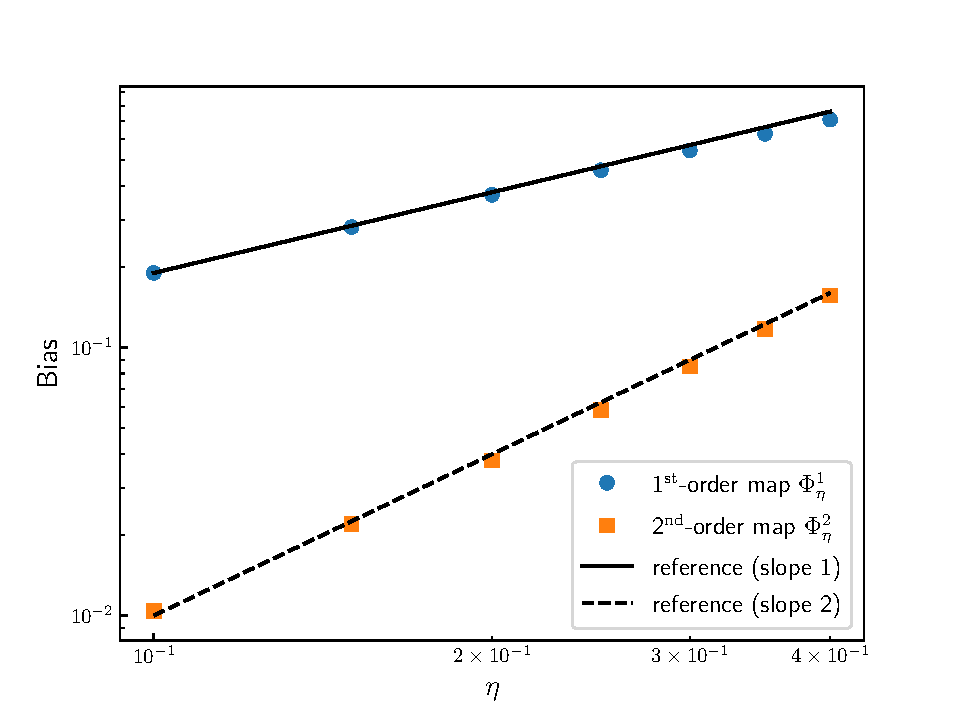
\includegraphics[width=0.75\textwidth]{1d-lang_bias.pdf}
	\caption{Bias \eqref{eq:bias_1d-lang} as a function of $\eta$ for the first and second-order maps, with overlayed reference lines.}
	\label{fig:1d_lang_bias}
\end{figure}

% ===================================================================================
\subsection{Mobility and shear viscosity for Lennard--Jones fluids}
\label{subsec:num_LJ}
%
We next present some numerical results highlighting the variance-reduction potential of the transient subtraction method. The example in consideration is the computation of shear viscosity and mobility for a Lennard--Jones fluid. The system in consideration is composed of $N$ particles in spatial dimension $D=3$ (so that~$d=DN$), evolving according to the underdamped Langevin dynamics \eqref{eq:lang_dynamics}. The potential energy corresponds to the sum of pairwise interactions
%
\begin{equation}
	V(q) = \sum_{1\leq i<j\leq N} v(\norm{q_i - q_j}),
\end{equation}
%
with $v(r)$ given by the standard 12-6 Lennard--Jones interaction potential:
%
\begin{equation}
	v(r) = 4\eps\bkt*{\paren*{\frac{\sigma}{r}}^{12} - \paren*{\frac{\sigma}{r}}^6}.
	\label{eq:LJ_pairwise}
\end{equation}
%
The parameter $\varepsilon$ represents the depth of the potential well, and $\sigma$ is the distance at which interactions are 0, i.e.\ when interactions go from attractive to repulsive. In practice, one truncates the range of~\eqref{eq:LJ_pairwise} at some value $r_\mathrm{c}$, after which interactions can be deemed negligible. We employ the truncated shifted-force cutoff method with a cutoff value of $r_\mathrm{c}=2.5\sigma$, resulting in the modified potential
%
\begin{equation}
	v_\mathrm{SF}(r) = [v(r) - v(r_\mathrm{c}) - (r - r_\mathrm{c})v'(r_\mathrm{c})]\ind_{r\leq r_\mathrm{c}}.
\end{equation}
%  
We numerically integrate the dynamics using the BAOAB splitting scheme. The simulations were conducted using with the \texttt{Molly.jl} package \cite{greener2024} in the Julia language, and were performed in dimensionless reduced units with $\sigma = \varepsilon = k_B = 1$ and the mass matrix~$M = \mathrm{Id}$. For both shear viscosity and mobility computations, the results we present correspond to averages over $10^5$ realizations of the system with i.i.d.\ initial conditions. 

We next describe the strategy for initializing and evaluating the trajectories, which is the procedurally identical for the mobility and shear cases. Each independent realization of the system is initialized as follows. For the equilibrium control system, initial momenta were sampled from the Boltzmann--Gibbs measure, while initial positions were initialized on a uniform grid. The system was then evolved for a thermalization time of $T_\mathrm{therm} = 1$ with a timestep size $\Delta t=10^{-3}$ in reduced units. We ensured that the thermalization time was sufficient long to melt the crystal structure and relax the system to a stationary-state, as monitored by the stabilization of kinetic and potential energies, and by visual inspection of the molecular structure. Next, we initialize the transient trajectory by applying the transformation \eqref{eq:LJ_gen_map} to a copy of the stationary equilibrium system:
%
\begin{align}
    \begin{pmatrix}
        q_0^\eta \\ p_0^\eta
    \end{pmatrix}
	 = \Phi_\eta(q_0^0,p_0^0) = 
	\begin{pmatrix}
 	  q_0^0 \\ p_0^0 + \eta F(q_0^0)
 	\end{pmatrix},
 	\label{eq:LJ_gen_map}
\end{align}
%
where the expression for $F(q)$ is made precise for mobility and shear viscosity in \cref{subsubsec:mobility_num,subsubsec:shear}, respectively. The equilibrium and transient trajectories are then evolved simultaneously according to synchronously coupled standard equilibrium dynamics. The integration time $T$ should not be much larger than the relaxation time of the transient trajectory, as decoupling becomes a significant source of error. Nevertheless, this can be overcome during postprocessing, during which one can choose the appropriate truncation time for the estimator. Observational runs should be performed beforehand to ensure that one knows the approximate relaxation time (which varies significantly depending on the system at hand), which can be deduced from reasonably coarse and inexpensive runs. All simulation parameters are made precise in \cref{table:sim_params}.
%
%The simulations were performed in dimensionless reduced units, with reference values given by the Lennard--Jones parameters $\sigma,\varepsilon$, the Boltzmann constant $k_B$ and the mass $M$, all set to 1. We employ the shifted-force cutoff method for truncating the potential with a cutoff value with a cutoff value of $r_\mathrm{c}=2.5$. The resulting expression for the potential reads
%%
%\begin{equation}
%	v_\mathrm{SF}(r) = [v(r) - v(r_\mathrm{c}) - (r - r_\mathrm{c})v'(r_\mathrm{c})]\ind_{r\leq r_\mathrm{c}}.
%\end{equation}
%%
%We compute the shear viscosity and mobility for a Lennard--Jones fluid as described above. The simulations were performed in the Julia language using with the \texttt{Molly.jl} package \cite{greener2024}. We numerically integrate the dynamics using the BAOAB splitting scheme. All other simulation parameters are made precise in \cref{table:sim_params}.
%
\begin{table}[h!]
\begin{center}
	\begin{tabular}{lcc} 
	\toprule
	\bf{Parameter} & {\bf Shear visc.} & {\bf Mobility} \\
	\midrule
%	Perturbation $\eta$ & $10^{-2}$ & $10^{-2}$ \\
    Integration time ($T$) & 3.5 & 2.0 \\
    Thermalization time ($T_\mathrm{therm}$) & 1 & 1 \\
	No. of realizations ($K$) & $10^5$ & $10^5$ \\
	Timestep ($\Delta t$) & $10^{-3}$ & $10^{-3}$ \\
	Inverse temp. ($\beta$) & 1.25 & 0.8 \\
	Damping ($\gamma$) & 1 & 1 \\
	No. of particles ($N$) & 1000 & 1000 \\
	Particle density ($\varrho$ [$N$/vol.]) & 0.7 & 0.6 \\
	LJ cutoff ($r_\mathrm{c}$) & 2.5 & 2.5 \\
	Mass matrix $M$ & {\rm Id} & {\rm Id} \\
	LJ param. $(\sigma)$ & 1 & 1 \\
	LJ param. $(\varepsilon)$ & 1 & 1 \\
	Boltzmann const. ($k_B$) & 1 & 1 \\
	\bottomrule
	\end{tabular}
\end{center}
\caption{Simulation parameters}
\label{table:sim_params}
\end{table}

\subsubsection{Mobility}
\label{subsubsec:mobility_num}
%
When under the effect of a constant external field $F$, the mobility quantifies the particles' drift velocity in the direction of the applied field. In our Lennard--Jones fluid example, we consider a constant force applied in the $x$-direction, and in particular we consider colored drift, which amounts to perturbing half the particles to one direction, and the other half in the opposite direction:
%
\begin{equation}
	F = \frac{1}{\sqrt{N}}(F_1,F_2,\dotsc,F_N)^\t \in \R^{3N}, \qquad F_i = ((-1)^{i+1}, 0, 0), \qquad i = 1,\dotsc,N.
\end{equation}
%
The observable we consider is the velocity in the direction $F$, and is the standard choice for mobility computations \cite[Section 5.2.2]{lelievre2016}:
%
\begin{equation}
	R(q,p) = F^\t M^{-1}p.
\end{equation}
%
%\begin{align}
%    (q_0^\eta, p_0^\eta) = \Phi_\eta(q_0^0, p_0^0) = (q_0^0, p_0^0 + \eta F)
%\end{align}
%
\begin{figure}[h!]
\centering
\begin{subfigure}{0.49\textwidth}
    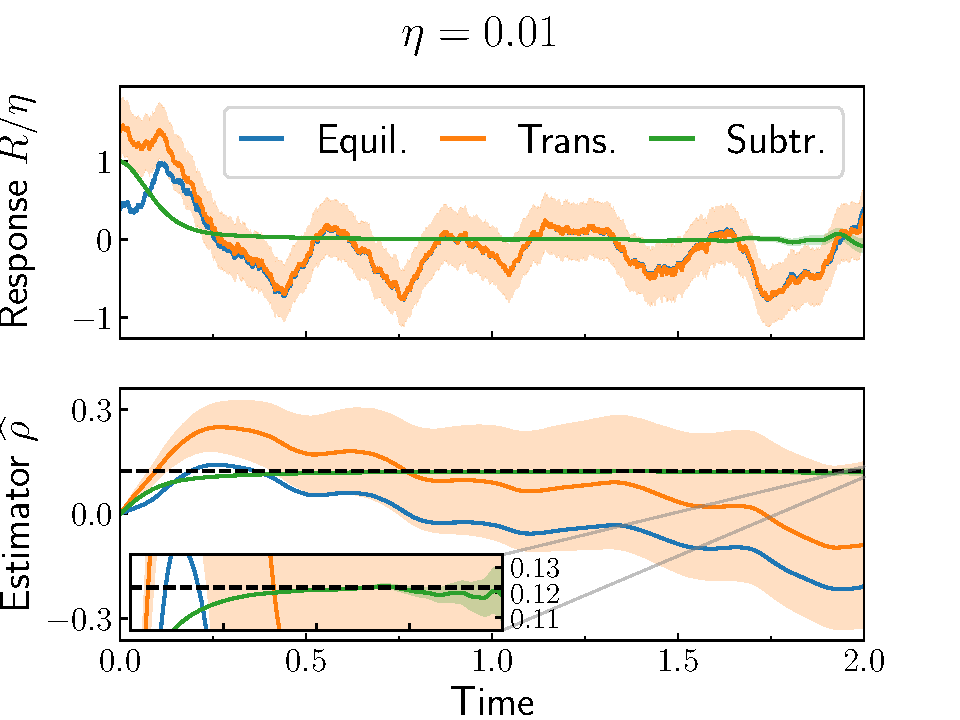
\includegraphics[width=\textwidth]{LJ_mobility_0.01.pdf}
    \caption{Data for $\eta = 0.01$.}
    \label{subfig:mobility_0.01}
\end{subfigure}
\hfill
\begin{subfigure}{0.49\textwidth}
    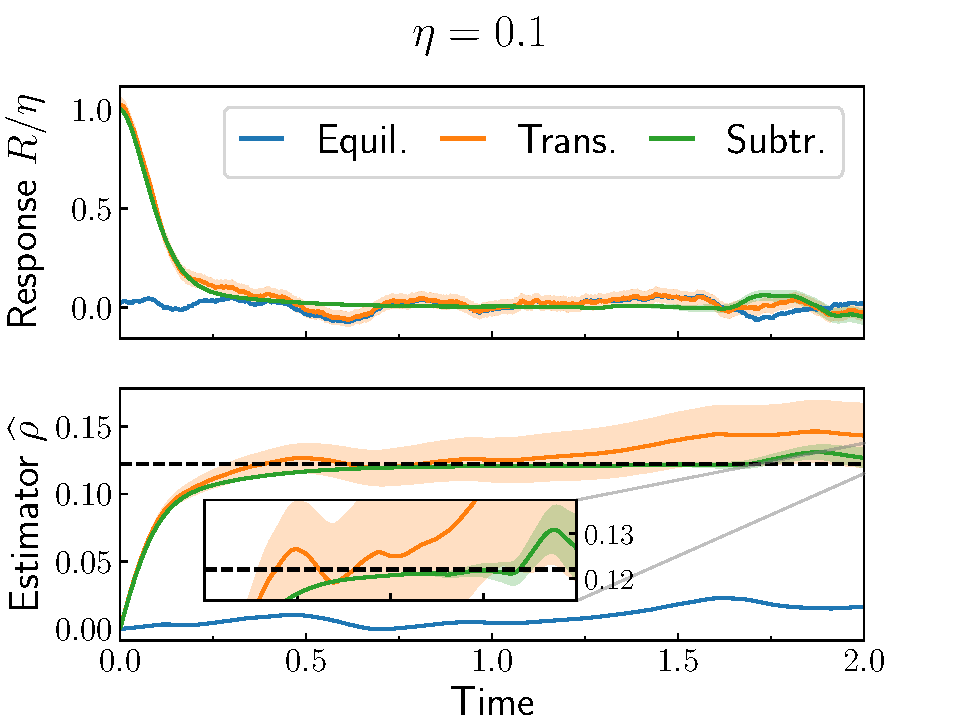
\includegraphics[width=\textwidth]{LJ_mobility_0.1.pdf}
    \caption{Data for $\eta = 0.1$.}
    \label{subfig:mobility_0.1}
\end{subfigure}
\caption{Trajectories for the computation of the mobility of a Lennard--Jones fluid with colored drift and associated error bars. The top graphs correspond to the instantaneous response (normalized by~$\eta$) as a function of time as transient trajectory relaxes, while the bottom graphs show the integrated response over time.}
\label{fig:LJ_mobility}
\end{figure}
%
\begin{table}[h!]
%\centering
\begin{subtable}[h]{0.45\textwidth}
\centering
\begin{tabular}{lccc}
\toprule
 & \multicolumn{2}{c}{\textbf{Variance at $T=1$}} &  \\
\cmidrule(lr){2-3}
 $\eta$ & \textbf{Naive} & \textbf{Subtraction} & \textbf{Ratio} \\
\midrule
%0.01 & 2660.7629 & 0.00469 & 566650.8213 \\
%0.1  & 26.5611   & 0.00465 & 5712.2716  \\
%1.0  & 0.2647    & 0.00437 & 60.5459    \\
0.01 & $\sn{2.66}{3}$ & $\sn{4.69}{-3}$ & $\sn{5.67}{5}$ \\
0.1  & 26.6   & $\sn{4.65}{-3}$ & $\sn{5.71}{3}$  \\
1.0  & 0.265    & $\sn{4.37}{-3}$ & 60.6    \\
\bottomrule
\end{tabular}
\caption{Data at $T=1$ (start of decoupling)}
\end{subtable}%
\hfill
\begin{subtable}[h]{0.45\textwidth}
\centering
\begin{tabular}{lccc}
\toprule
 & \multicolumn{2}{c}{\textbf{Variance at $T=2$}} &  \\
\cmidrule(lr){2-3}
 $\eta$ & \textbf{Naive} & \textbf{Subtraction} & \textbf{Ratio} \\
\midrule
%0.01 & 5700.3092 & 11.7473 & 485.2457 \\
%0.1  & 57.1811   & 5.5182  & 10.3622  \\
%1.0  & 0.5644    & 0.2859  & 1.9740   \\
0.01 & $\sn{5.70}{3}$ & 11.8 & 485 \\
0.1  & 57.2   & 5.52  & 10.4  \\
1.0  & 0.564    & 0.286  & 1.97   \\
\bottomrule
\end{tabular}
\caption{Data at final time $T=2$ (total decoupling)}
\end{subtable}
\caption{Comparison of variances between naive and subtraction transient estimators for various values of $\eta$ for the computation of mobility.}
\label{table:LJ_mobility}
\end{table}
%
Each trajectory is integrated for a physical time $T=2$. Although the system relaxes significantly before, we deliberately wanted to observe the decoupling point, which can be easily spotted in \cref{fig:LJ_mobility}, which shows the average trajectories for two values of $\eta$. Due to the large signal-to-noise ratio of the mobility response, the subtraction's uniform bound in $\eta$ of the variance indeed shows to make a difference, as can readily be seen from \cref{fig:LJ_mobility}. The associated error bars shown in \cref{fig:LJ_mobility} were computed with empirical averages over the independent realizations.

To quantitatively assess the variance reduction and the decoupling effect, we consider the variance values for both the naive transient and subtraction methods at two different times $T$: one right before trajectories decouple $T=1$, and one at the final time $T=2$. These results are summarized in \cref{table:LJ_mobility}. At $T=1$, we indeed see the variance's uniform bound in $\eta$ for the subtraction trajectory, while the $\eta^{-2}$ factor shows for the naive trajectory. Additionally, we notice that at $T=2$, even after significant decoupling after decoupling, the subtraction method still provides significant variance reduction, even long after relaxation has occured.

\subsubsection{Shear viscosity}
\label{subsubsec:shear}
%
The shear viscosity of a fluid can be computed in a variety of ways; see \cite{todd2007} for a review on computational techniques. In this work, we consider a setting based on the transverse force-field method \cite{joubaud2012} with a sinusoidal forcing profile. We denote by $F_i\in\R^3$ the force acting on the $i$th particle:
%
\begin{equation}
    F_i = (f(q_y), 0, 0)^\t, \qquad  f(y) = \sin\paren*{\frac{2\pi y}{L_y}}.
\end{equation}
%
The force acts on the $x$-component of the momenta based on the particle's $y$-coordinate position.
%
%\begin{equation}
%	\nu = \varrho\paren*{\frac{1}{2\rho} - \gamma_x}\paren*{\frac{L_y}{2\pi}}^2
%\end{equation}
%%
%
%
The observable $R$ of interest is the imaginary part of the first empirical Fourier coefficient $U_1$:
%
\begin{equation}
    R(q,p) = \Im(U_1), \qquad U_1 = \frac{1}{N}\sum_{n=1}^N (M^{-1}p)_{n,x}\exp\paren*{\frac{2\mathrm{i}\pi q_{n,y}}{L_y}}.
    \label{eq:shear_observable}
\end{equation}
%
The initialization and evaluation of trajectories for this system were performed as described in \cref{subsec:num_LJ}. We consider the same numerical results as shown in \cref{subsubsec:mobility_num}, with largely the same interpretations and conclusion. A first difference, clearly seen from \cref{fig:LJ_shear}, however, is the magnitude of the error for the naive trajectories. This is a trivial artifact of the observable $R(q,p)$: for the mobility, the observable is $\bigO(\sqrt{N})$, while it is $\bigO(1)$ for the shear case, since \eqref{eq:shear_observable} corresponds to some spatial averaging. Secondly, the relaxation time for the shear trajectories is significantly longer compared to the one for mobility, and in fact almost coincides with the decoupling time. Nonetheless, \cref{table:LJ_shear} shows that variance reduction is still obtainable.
%
%\begin{align}
%    (q_0^\eta, p_0^\eta) = \Phi_\eta(q_0^0, p_0^0) = (q_0^0, \eta F(q_0^0))
%\end{align}

\begin{figure}[h!]
\centering
\begin{subfigure}{0.49\textwidth}
    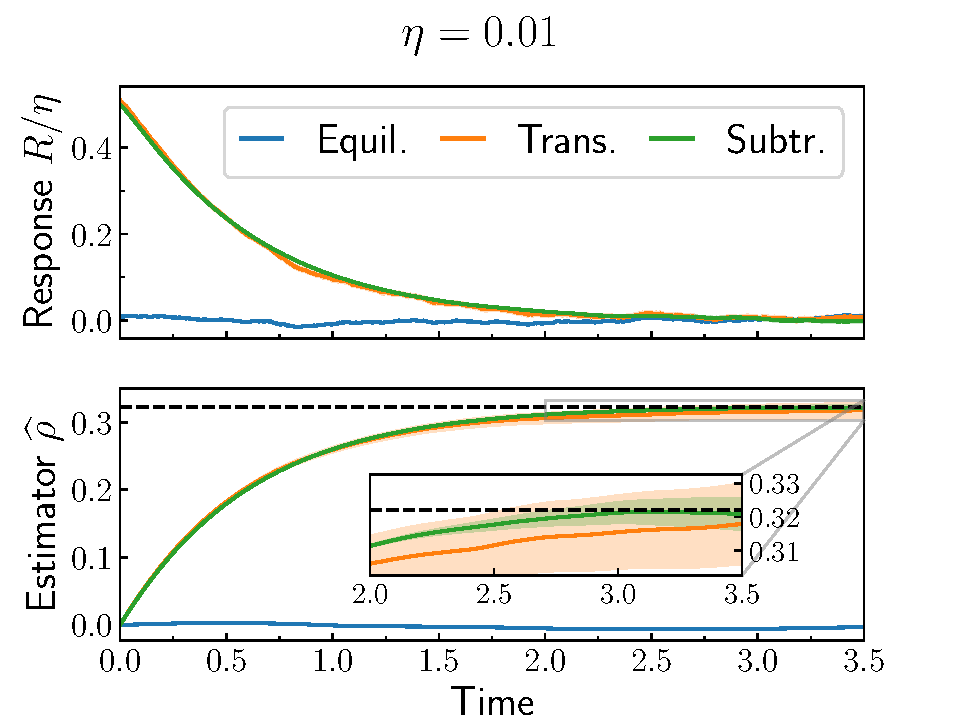
\includegraphics[width=\textwidth]{LJ_shear_0.01.pdf}
    \caption{Data for $\eta = 0.01$.}
    \label{subfig:shear_0.01}
\end{subfigure}
\hfill
\begin{subfigure}{0.49\textwidth}
    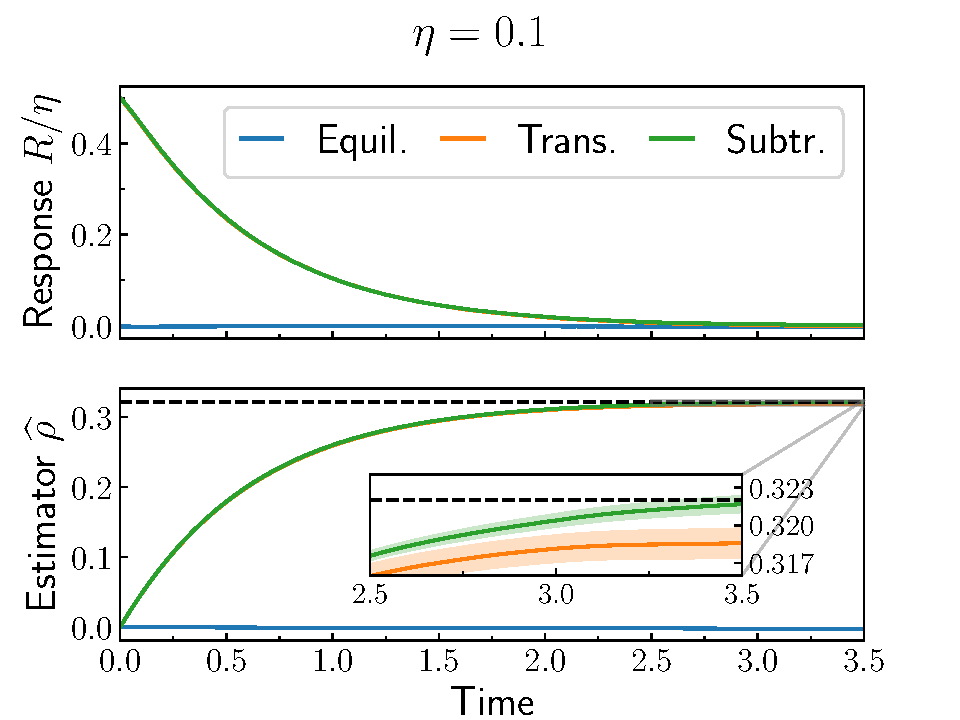
\includegraphics[width=\textwidth]{LJ_shear_0.1.pdf}
    \caption{Data for $\eta = 0.1$.}
    \label{subfig:shear_0.1}
\end{subfigure}
\caption{Trajectories for the computation of the shear viscosity of a Lennard--Jones fluid and associated error bars. The top graphs correspond to the instantaneous response (normalized by~$\eta$) as a function of time as transient trajectory relaxes, while the bottom graphs show the integrated response over time.}
\label{fig:LJ_shear}
\end{figure}

\begin{table}[h!]
%\centering
\begin{subtable}[h]{0.45\textwidth}
\centering
\begin{tabular}{lccc}
\toprule
 & \multicolumn{2}{c}{\textbf{Variance at $T=2$}} &  \\
\cmidrule(lr){2-3}
% $\eta$ & \textbf{Naive } & \textbf{Subtraction } & \textbf{Ratio} \\
 $\eta$ & \textbf{Naive } & \textbf{Subtraction } & \textbf{Ratio} \\
\midrule
%0.01 & 7.32049 & 0.02604 & 281.07928 \\
%0.1 & 0.07262 & 0.0054957 & 13.21505 \\
0.01 & 7.32 & 0.0260 & 281 \\
0.1 & 0.0726 & $\sn{5.49}{-3}$ & 13.2 \\
\bottomrule
\end{tabular}
\caption{Data at $T=2$ (start of decoupling)}
\end{subtable}%
\hfill
\begin{subtable}[h]{0.45\textwidth}
\centering
\begin{tabular}{lccc}
\toprule
 & \multicolumn{2}{c}{\textbf{Variance at $T=3.5$}} &  \\
\cmidrule(lr){2-3}
 $\eta$ & \textbf{Naive } & \textbf{Subtraction } & \textbf{Ratio} \\
\midrule
%0.01 & 14.9814 & 2.4468 & 6.1229 \\
%0.1  & 0.1497  & 0.0487 & 3.0730 \\
0.01 & 15.0 & 2.45 & 6.12 \\
0.1  & 0.150  & 0.0487 & 3.07 \\
\bottomrule
\end{tabular}
\caption{Data at final time $T=3.5$ (total decoupling)}
\end{subtable}
\caption{Comparison of variances between naive and subtraction transient estimators for various values of $\eta$ for the computation of shear viscosity.}
\label{table:LJ_shear}
\end{table}